\section{Widget testing}
Widget testing aims to test UI behavior to certain actions and it's not about functionalities and logic like the unit testing.
This type of testing is made available thanks to a \textit{Widget tester} library embedded in the flutter SDK.
\newline
\newline
\noindent The main widget tested were the sign up, sign in and the add modal product.
\newline
\newline
\noindent There it presents once again the need of using stubs because of internal dependencies inside screens and widget. The difference with the unit testing is the impossibility to perform a large scale refactoring since implementing an injectable constructor would be a tedious and very long task. We solved this by using a \textit{dependencies provider} that is responsible for providing dependencies to each widget requiring it. By doing this, each widget has dependencies fetching completely transparent while we can inject the dependencies provider with mocks to be served to widgets.

\begin{center}
    \vspace{1cm}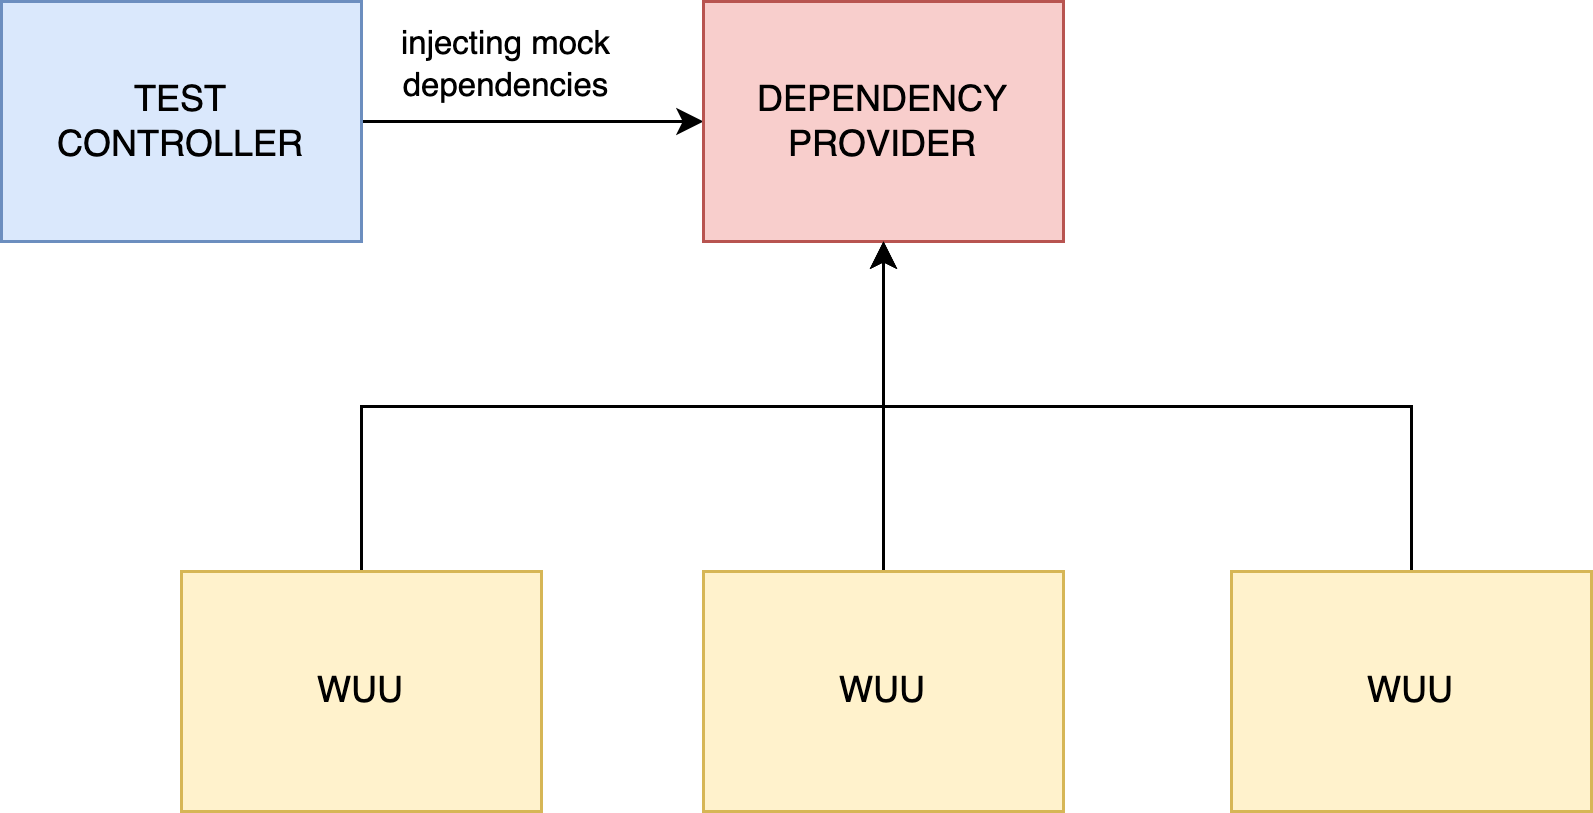
\includegraphics[width=12cm,keepaspectratio]{Images/testing/widget_testing.png}
\end{center}


\newpage